% ============================================================================
%  UGP report: gas-bubble percolation on grain boundaries (phase-field)
%  Compile: pdflatex main.tex (twice), or upload this folder to Overleaf.
%  Figures: figures/  (regenerate with  python3 make_figures.py  from the data)
%  >>> Fill in the three XXXX macros below before submitting. <<<
% ============================================================================
\documentclass[11pt,a4paper]{article}

\newcommand{\studentname}{Gaurav Kumar}
\newcommand{\rollno}{Roll No.\ XXXXXXX}
\newcommand{\supervisor}{Prof.\ XXXXXXXX}
\newcommand{\department}{Department of XXXXXXXX, XXXXXXXX Institute}

\usepackage[T1]{fontenc}
\usepackage{lmodern}
\usepackage{microtype}
\usepackage[margin=2cm]{geometry}
\usepackage{amsmath,amssymb}
\usepackage{graphicx}
\usepackage{booktabs}
\usepackage{xcolor}
\usepackage{tikz}
\usepackage{tcolorbox}
\usepackage[font=small,labelfont=bf,skip=4pt]{caption}
\usepackage[compact]{titlesec}
\usepackage{enumitem}
\usepackage[hidelinks]{hyperref}
\graphicspath{{figures/}}
\setlist{nosep,leftmargin=*}
\setlength{\parskip}{3pt}
\setlength{\parindent}{0pt}
\titlespacing*{\section}{0pt}{9pt}{3pt}
\titlespacing*{\subsection}{0pt}{6pt}{2pt}

\definecolor{boxblue}{HTML}{2A78D6}
\newtcolorbox{takeaway}{colback=boxblue!5, colframe=boxblue!60, boxrule=0.5pt,
  arc=2pt, left=6pt, right=6pt, top=3pt, bottom=3pt, fontupper=\small}

\newcommand{\Atot}{A_{\mathrm{tot}}}
\newcommand{\bGB}{b_{GB}}

% ----------------------------------------------------------------------------
\begin{document}

\begin{center}
{\LARGE\bfseries When do gas bubbles on a grain boundary connect?}\\[4pt]
{\large A phase-field study of bubble percolation in irradiated materials}\\[8pt]
Undergraduate Project (UGP) Report\\[4pt]
\studentname\quad(\rollno)\qquad Supervisor: \supervisor\\
\department\qquad November 2026
\end{center}

\begin{abstract}
\noindent
\textbf{Problem.} Irradiation creates gas atoms (He, Xe, Kr) that collect on
grain boundaries (GBs) as small bubbles. As the bubbles grow they touch and
join. When they form one connected network (\emph{percolation}), gas can escape
and the boundary becomes weak. We want to know at what \emph{coverage} (fraction
of the GB covered by bubbles) this happens, and what controls it.
\textbf{What we did.} We wrote a 3-D phase-field code (Cahn--Hilliard equation
for the gas, Allen--Cahn equations for the grains). We first studied one bubble
and used it to fix the simulation parameters. We then grew 33 and 25 bubbles on
one GB, changed the contact angle $\theta$ (via the GB energy), and tracked how
the bubbles join. Finally we made the GB move and repeated the test.
\textbf{Main findings.} (1) Percolation starts at the same coverage (0.39 for 33
bubbles) for every contact angle, and ends at the same coverage (0.70--0.72) for
the angles that reach the end; the angle mainly changes \emph{how fast} this
happens (3.4$\times$). (2) Fewer bubbles shift both values to lower coverage.
(3) Very round bubbles ($\theta\ge128^\circ$) stop joining. (4) A moving GB is
not pinned by the bubbles; it drags them along. (5) The percolation curve is the
same whether the GB moves or not.
\end{abstract}

% ----------------------------------------------------------------------------
\section{The problem}

Under irradiation, materials produce gas atoms that do not dissolve in the
crystal: xenon and krypton in nuclear fuel, helium in structural
steels~\cite{Trinkaus2003,Tonks2018}. These atoms move to grain boundaries and
form bubbles there. A GB bubble looks like a lens (Fig.~\ref{fig:sketch}a). Its
shape is set by the \emph{contact angle} $\theta$, which comes from a balance of
the GB energy $\gamma_{GB}$ and the bubble surface energy
$\gamma_s$: $\gamma_{GB}=2\gamma_s\cos(\theta/2)$. A higher GB energy gives a
smaller $\theta$ and a flatter lens.

As more gas arrives, the lenses grow, touch and merge. At some point they form
one connected cluster. This is \emph{percolation}, and it matters because gas can
then vent out (fission gas release) and the boundary loses strength. Fuel
models often assume that it happens at a fixed coverage~\cite{White2004,Tonks2018}.
In this project we asked: \emph{does the coverage at percolation depend on the
contact angle, on the number of bubbles, or on whether the GB is moving?}

\begin{figure}[t]
\centering
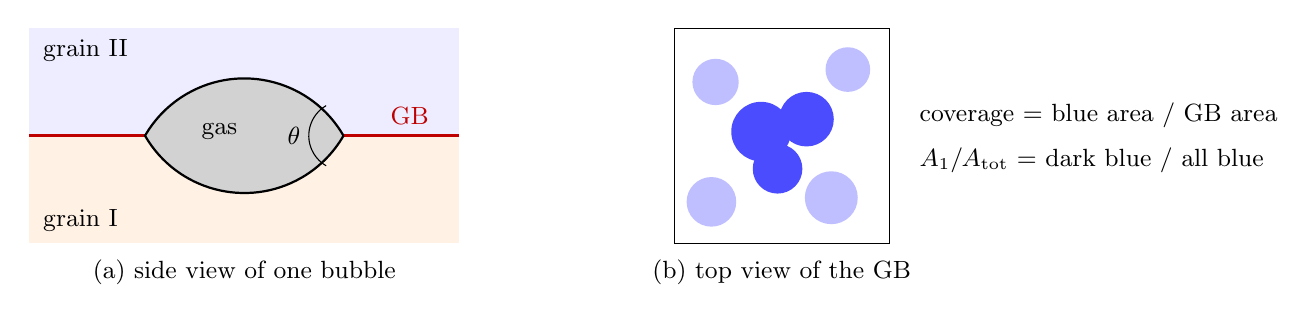
\begin{tikzpicture}[scale=1.05]
  % ---- (a) lens on a GB (side view), theta = 120 deg
  \fill[orange!10] (-2.6,-1.3) rectangle (2.6,0);
  \fill[blue!7] (-2.6,0) rectangle (2.6,1.3);
  \draw[red!75!black, very thick] (-2.6,0) -- (-1.2,0);
  \draw[red!75!black, very thick] (1.2,0) -- (2.6,0);
  \fill[gray!35] (1.2,0) arc[start angle=30, end angle=150, radius=1.386]
                         arc[start angle=210, end angle=330, radius=1.386];
  \draw[thick] (1.2,0) arc[start angle=30, end angle=150, radius=1.386]
                       arc[start angle=210, end angle=330, radius=1.386];
  \draw[thin] (1.2,0) ++(120:0.42) arc[start angle=120, end angle=240, radius=0.42];
  \node at (0.6,0) {\small $\theta$};
  \node at (-0.3,0.05) {\small gas};
  \node[anchor=north west] at (-2.55,1.28) {\small grain II};
  \node[anchor=south west] at (-2.55,-1.28) {\small grain I};
  \node[red!75!black, anchor=south] at (2.0,0.02) {\small GB};
  \node at (0,-1.65) {\small (a) side view of one bubble};
  % ---- (b) top view of the GB plane
  \begin{scope}[xshift=5.2cm, yshift=-1.3cm]
    \draw[fill=white] (0,0) rectangle (2.6,2.6);
    \fill[blue!25] (0.45,0.5) circle (0.3);
    \fill[blue!25] (1.9,0.55) circle (0.32);
    \fill[blue!25] (0.5,1.95) circle (0.28);
    \fill[blue!25] (2.1,2.1) circle (0.27);
    \fill[blue!70] (1.05,1.35) circle (0.36);
    \fill[blue!70] (1.6,1.5) circle (0.33);
    \fill[blue!70] (1.25,0.9) circle (0.3);
    \node[anchor=west, align=left, font=\small] at (2.85,1.55)
      {coverage $=$ blue area / GB area};
    \node[anchor=west, align=left, font=\small] at (2.85,1.0)
      {$A_1/\Atot$ $=$ dark blue / all blue};
    \node at (1.3,-0.35) {\small (b) top view of the GB};
  \end{scope}
\end{tikzpicture}
\caption{(a)~A gas bubble sits on the GB as a lens; $\theta$ is the contact
angle. (b)~Looking down on the GB: the \emph{coverage} is the fraction covered
by bubbles, and $A_1/\Atot$ is the area of the largest connected bubble divided
by the total bubble area. $A_1/\Atot$ jumps towards 1 when the bubbles
percolate.}
\label{fig:sketch}
\end{figure}

% ----------------------------------------------------------------------------
\section{The model in brief}

We follow the phase-field model of Millett et al.~\cite{Millett2012}. Three
fields describe the material: the gas concentration $c$ ($c\approx1$ inside a
bubble, $c\approx0$ in the grains) and one order parameter per grain, $n_1$ and
$n_2$ ($n_1=1$ in grain I, $n_2=1$ in grain II). The free energy is
\begin{equation}
  F=\int\Big[A_0 f+\tfrac{\kappa}{2}\big(|\nabla c|^2+|\nabla n_1|^2+|\nabla n_2|^2\big)\Big]dV,\quad
  f=\tfrac{c^4}{4}-\tfrac{c^2}{2}+\sum_{i}\Big(\tfrac{n_i^4}{4}-\tfrac{n_i^2}{2}\Big)
    +\tfrac{\bGB}{2}n_1^2n_2^2+b_S\,c^2(n_1^2+n_2^2).
\end{equation}
The gas is conserved, so it follows the Cahn--Hilliard
equation~\cite{CahnHilliard1958}; the grains follow the Allen--Cahn
equation~\cite{AllenCahn1979}:
\begin{equation}
  \frac{\partial c}{\partial t}=\nabla\cdot\Big(M\,\nabla\frac{\delta F}{\delta c}\Big),\qquad
  \frac{\partial n_i}{\partial t}=-L_{GB}\,\frac{\delta F}{\delta n_i},\qquad
  M=16M_s c^2(1-c^2)+16M_{gb}n_1^2n_2^2+M_b .
\end{equation}
The mobility $M$ has three parts: diffusion along the bubble surface ($M_s$),
along the GB ($M_{gb}$) and through the bulk ($M_b$). The code is written in
C++ (OpenMP), uses finite differences on a $128\times128\times64$ grid, and
conserves gas to $10^{-13}$. \textbf{The ``knobs'' we turn} are:
\begin{itemize}
  \item \textbf{GB energy} $\bGB=1.2,\,1.5,\,2.0,\,3.0$, which gives contact angles
        $\theta=148^\circ,\,128^\circ,\,120^\circ,\,104^\circ$ (measured, $\pm6^\circ$).
        Only $\bGB$ is changed, so nothing else in the model changes;
  \item \textbf{gas and bubbles}: gas in the matrix $c_0$, starting bubble size
        $r_0$, number of bubbles $N$;
  \item \textbf{kinetics}: the mobilities $M_s$, $M_{gb}$ and the GB mobility $L_{GB}$;
  \item \textbf{a driving force} $\Delta f$ that makes the GB move (Sections~\ref{sec:flat}--\ref{sec:coupled}).
\end{itemize}
Fixed values: $A_0=4$, $b_S=1$, $\kappa=2$, $M_s=0.05$, $M_{gb}=0.5$, $M_b=5$,
$L_{GB}=1$. All lengths are in grid cells and all times are dimensionless.

% ----------------------------------------------------------------------------
\section{Step 1: one bubble on the GB}
\label{sec:single}

\textbf{What we did.} Before simulating many bubbles we studied a single one,
for two reasons: to see its shape for each contact angle, and to choose safe
values for the starting size $r_0$ and the gas content $c_0$.

\textbf{What we saw} (Fig.~\ref{fig:single}).
\begin{itemize}
  \item \emph{Shape.} When it settles, the bubble is a lens. A higher GB energy
        makes it flatter: $\theta$ drops from $148^\circ$ to $104^\circ$, in line
        with the force-balance formula.
  \item \emph{A minimum size.} Bubbles that start with $r_0\le3.0$ cells
        dissolve. $r_0=3.4$ just survives without growing, and $r_0\ge3.8$
        grows. The critical radius is therefore about 3.4--3.8 cells, and we
        used $r_0=4.5$ to be safely above it.
  \item \emph{Flat bubbles grow faster.} With the same start ($r_0=4.5$), the
        flat $104^\circ$ bubble reaches 1.7 times the volume of the round
        $148^\circ$ bubble by $t=10$ (2138 vs 1252 cells).
  \item \emph{Gas content.} With $c_0=0.30$ the bare GB itself filled with a gas
        film, even with no bubble present. $c_0=0.12$ is the largest value for
        which this never happens at any of the four angles, so we used it.
  \item \emph{Kinetics.} Switching off surface and GB diffusion ($M_s=M_{gb}=0$)
        changed every result by less than 1\,\%. The gas travels mainly through
        the bulk.
\end{itemize}

\begin{figure}[t]
\centering
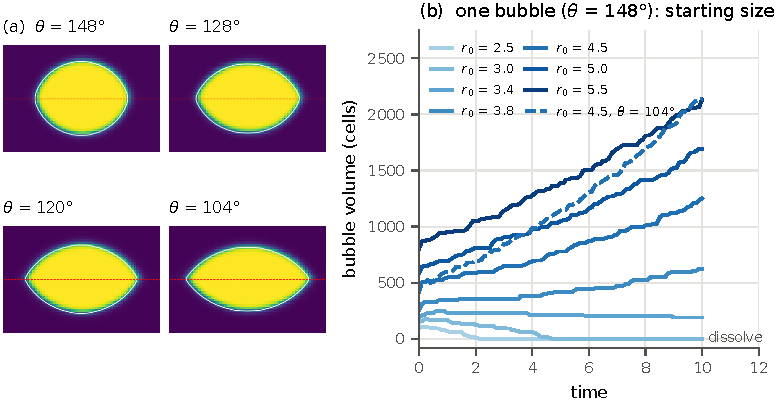
\includegraphics[width=\textwidth]{f1_single.pdf}
\caption{One bubble on the GB. (a)~Settled lens shapes for the four GB energies
(yellow: gas; red dashed: GB). (b)~Bubble volume over time for different
starting radii at $\theta=148^\circ$ (solid); small bubbles dissolve, large ones
grow. Dashed: $r_0=4.5$ at $\theta=104^\circ$, which grows faster.}
\label{fig:single}
\end{figure}

\begin{takeaway}
\textbf{Take-away.} A bubble must start above about 3.5 cells to grow, and
flatter (low-$\theta$) bubbles grow faster. From this step we fixed $r_0=4.5$
and $c_0=0.12$, and learned that bulk diffusion controls the growth.
\end{takeaway}

% ----------------------------------------------------------------------------
\section{Step 2: many bubbles and percolation}
\label{sec:perc}

\textbf{What we did.} We placed $N=33$ bubbles ($r_0=4.5$) at random positions
on a flat GB that does not move, with $c_0=0.12$ of gas in the grains and no
extra gas source. Then we let them grow and join. We repeated this for the four
contact angles, and for $N=25$ (the first 25 of the same 33 positions, so the
two layouts can be compared directly). Runs stop when only one bubble is left,
or at $t=150$.

\textbf{What we measured, and why.} Looking down on the GB
(Fig.~\ref{fig:sketch}b), we recorded every 0.1 time units:
\begin{itemize}
  \item the \emph{coverage}: how much of the GB is under bubbles. This is the
        quantity fuel models use;
  \item the \emph{number of separate bubbles}. Its first drop marks the
        \textbf{start of percolation} (first merger), and reaching 1 marks the
        \textbf{end} (one connected bubble);
  \item $A_1/\Atot$, the share of the largest bubble. It stays near $1/N$ while
        the bubbles are separate and jumps up as they connect, so it is the
        clearest picture of percolation.
\end{itemize}

\subsection{The first plot: largest bubble vs coverage}

Fig.~\ref{fig:a1} was the first plot we drew. For all angles, $A_1/\Atot$ stays
flat until the coverage reaches about 0.39 ($N=33$) or 0.32 ($N=25$). It then
climbs in steps, each step being a merger, and reaches 1 at about 0.70 ($N=33$)
or 0.64 ($N=25$). The curves for different angles lie almost on top of each
other, especially for $104^\circ$ and $120^\circ$. The $128^\circ$ curve is
slightly to the right, and the $148^\circ$ curve stops early (discussed below).

\begin{figure}[t]
\centering
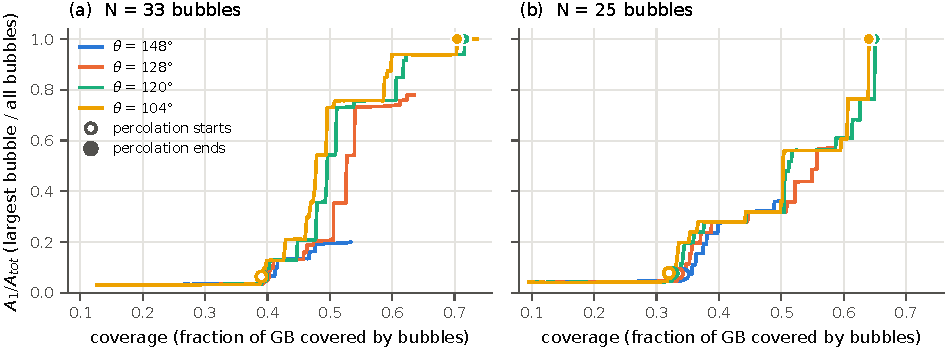
\includegraphics[width=\textwidth]{f2_a1_coverage.pdf}
\caption{Share of the largest bubble, $A_1/\Atot$, against coverage for the four
contact angles. Open circle: percolation starts; filled circle: percolation
ends (one bubble). The $128^\circ$ and $148^\circ$ curves are drawn up to their
highest coverage.}
\label{fig:a1}
\end{figure}

\subsection{What the bubbles look like}

Fig.~\ref{fig:morph} shows the GB from above. All four cases start from exactly
the same bubbles. Flat bubbles ($104^\circ$) spread sideways and touch early: at
$t=12$ they have already merged into 8 bubbles, while at $148^\circ$ all 33 are
still separate. The end states are very different. At $104^\circ$ and
$120^\circ$ the gas forms one connected network with holes. At $128^\circ$ and
$148^\circ$ a few thick, round islands remain; the colour shows they are up to
24 cells thick, against 12--14 at low angles.

\begin{figure}[t]
\centering
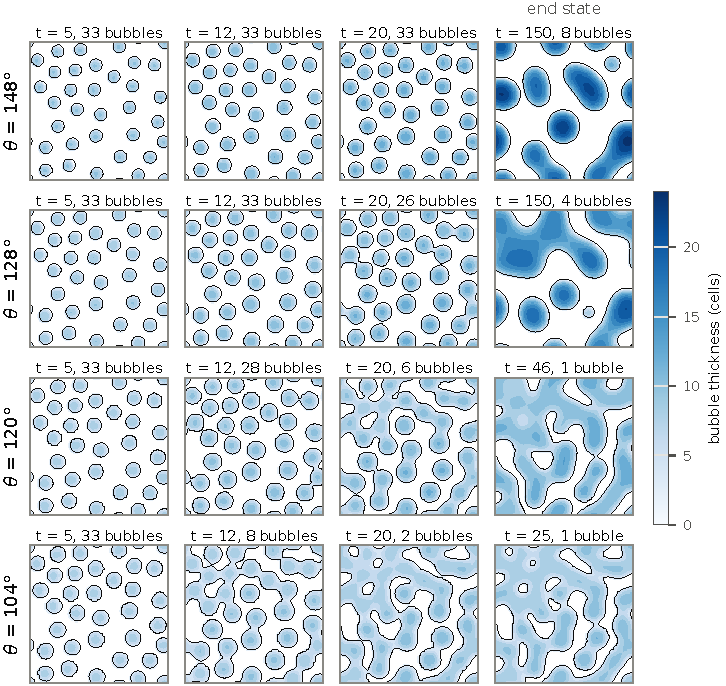
\includegraphics[width=0.76\textwidth]{f3_morphology.pdf}
\caption{Top view of the GB with 33 bubbles. Colour: bubble thickness; black
line: edge of the covered area. Rows: contact angle. Columns: $t=5$, 12, 20 and
the end state (one bubble, or $t=150$).}
\label{fig:morph}
\end{figure}

\subsection{Effect of contact angle and number of bubbles}

\begin{table}[b]
\centering
\caption{Coverage and time at the start (first merger) and end (one bubble) of
percolation. ``---'': not reached by $t=150$ (islands left in brackets).}
\label{tab:perc}
\small
\setlength{\tabcolsep}{5pt}
\begin{tabular}{c cc cc cc cc}
\toprule
 & \multicolumn{4}{c}{Percolation starts} & \multicolumn{4}{c}{Percolation ends}\\
\cmidrule(lr){2-5}\cmidrule(lr){6-9}
 & \multicolumn{2}{c}{$N=33$} & \multicolumn{2}{c}{$N=25$} & \multicolumn{2}{c}{$N=33$} & \multicolumn{2}{c}{$N=25$}\\
$\theta$ & coverage & $t$ & coverage & $t$ & coverage & $t$ & coverage & $t$\\
\midrule
$148^\circ$ & 0.394 & 27.6 & 0.344 & 26.7 & --- (8) & $>150$ & --- (6) & $>150$\\
$128^\circ$ & 0.394 & 16.9 & 0.334 & 16.6 & --- (4) & $>150$ & --- (4) & $>150$\\
$120^\circ$ & 0.392 & 11.3 & 0.326 & 11.2 & 0.716 & 45.6 & 0.650 & 55.7\\
$104^\circ$ & 0.390 &  8.0 & 0.320 &  7.9 & 0.704 & 24.1 & 0.640 & 29.6\\
\bottomrule
\end{tabular}
\end{table}

Table~\ref{tab:perc} and Fig.~\ref{fig:perc} give the numbers.
\begin{itemize}
  \item \textbf{Start, same coverage for every angle.} With 33 bubbles the first
        merger happens at coverage 0.390--0.394 for all four angles (only 1\,\%
        spread). The time changes a lot, from $t=8.0$ to 27.6 (3.4$\times$).
  \item \textbf{End, same coverage for the angles that get there.} $104^\circ$ and
        $120^\circ$ end as one bubble at almost the same coverage (0.704 and
        0.716), although one takes twice as long as the other ($t=24$ vs 46).
  \item \textbf{Fewer bubbles, lower coverage.} With 25 bubbles, percolation
        starts at 0.32--0.34 and ends at 0.64--0.65. Here the start rises
        slightly with angle (7\,\%).
  \item \textbf{Round bubbles stall.} At $128^\circ$ and $148^\circ$ the bubbles
        never become one, even by $t=150$ (5--6 times longer than $104^\circ$
        needed). Their coverage peaks (0.50--0.63) and then \emph{falls}, because
        the merged islands become rounder and thicker and pull back from their
        neighbours. The smallest gap between islands stops closing
        (Fig.~\ref{fig:perc}c,f). At $148^\circ$, five small islands simply
        dissolve into larger ones (Ostwald ripening) instead of merging.
\end{itemize}

\begin{figure}[t]
\centering
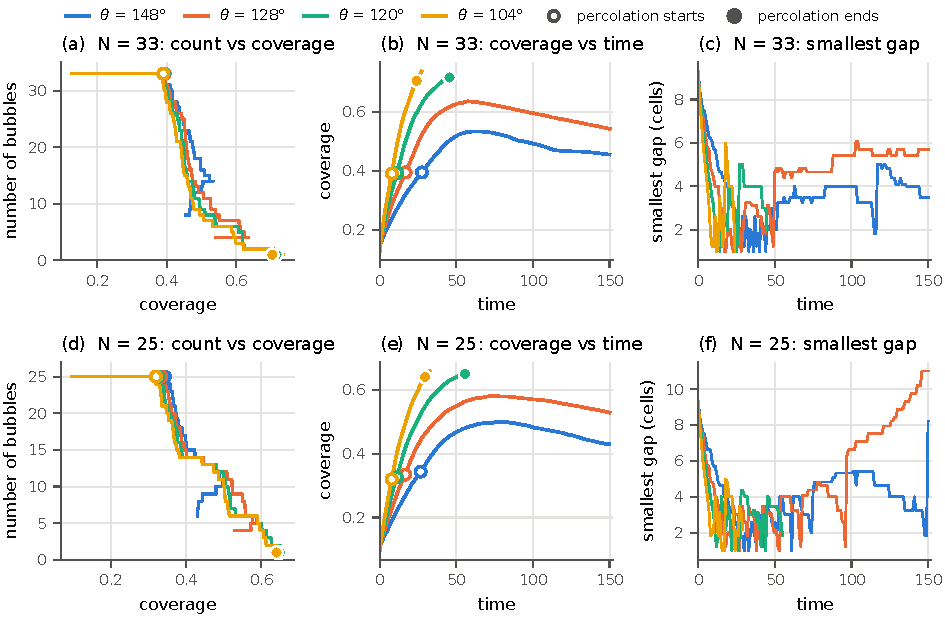
\includegraphics[width=\textwidth]{f4_percolation.pdf}
\caption{Percolation measurements for 33 bubbles (top) and 25 bubbles (bottom).
(a,d)~Number of bubbles vs coverage. (b,e)~Coverage vs time. (c,f)~Smallest gap
between two islands; at high angles it stops closing.}
\label{fig:perc}
\end{figure}

\begin{takeaway}
\textbf{Take-away.} For a given set of bubbles, percolation \emph{starts} at the
same coverage for every contact angle, and \emph{ends} at the same coverage for
every angle that reaches the end. The contact angle mainly decides \emph{when}
this happens, not \emph{at what coverage}. The number of bubbles does shift the
coverage. Very round bubbles ($\theta\ge128^\circ$) stop connecting.
\end{takeaway}

% ----------------------------------------------------------------------------
\section{Step 3: a flat GB that moves (no bubbles)}
\label{sec:flat}

\textbf{What we did.} Real GBs move, for example during grain growth. To make a
flat GB move, we gave grain II a slightly higher energy, $\Delta f$. Grain I
then grows into grain II and pushes the GB upward. We first checked this
without any gas, in a $32\times32\times64$ box, for $\Delta f=0$ to 0.1.

\textbf{What we saw} (Fig.~\ref{fig:flat}).
\begin{itemize}
  \item The GB moves at a steady average speed that grows with $\Delta f$:
        0.040, 0.068, 0.114 and 0.158 cells per unit time for $\Delta f=0.0375$,
        0.05, 0.075 and 0.1.
  \item The speed is 57--85\,\% of the theoretical value $v=1.865\,\Delta f$,
        getting closer at larger $\Delta f$. The GB moves in small jumps, once
        per grid cell.
  \item At $\Delta f\le0.025$ the GB moves 0.6 cells and then stops. It is
        \emph{pinned by the grid}, because the GB is only about 3 cells wide.
  \item A GB that starts with a small ripple flattens at the rate the theory
        predicts (0.0763 vs 0.0771), then moves like the flat GB.
\end{itemize}

\begin{figure}[t]
\centering
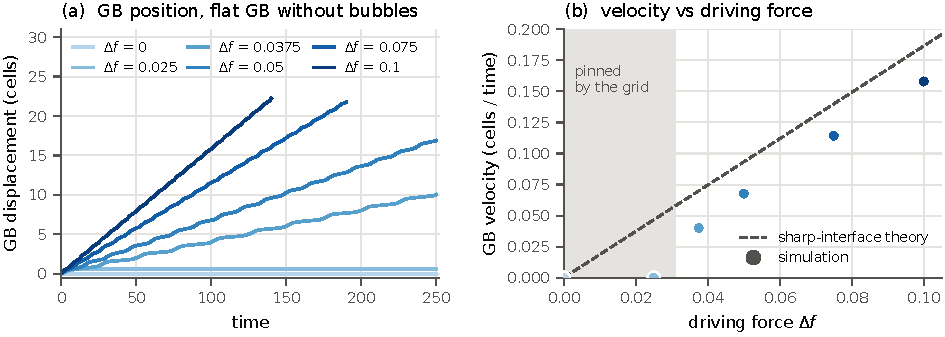
\includegraphics[width=\textwidth]{f5_flatgb.pdf}
\caption{A flat GB driven by an energy difference $\Delta f$, without bubbles.
(a)~Distance moved over time. (b)~Average speed vs $\Delta f$, compared with
the sharp-interface theory; below $\Delta f\approx0.03$ the GB is pinned by the
grid.}
\label{fig:flat}
\end{figure}

\begin{takeaway}
\textbf{Take-away.} The moving-GB set-up works: the speed is steady and
controlled by $\Delta f$. Because of grid pinning at small $\Delta f$, we used
$\Delta f\ge0.1$ in the next step.
\end{takeaway}

% ----------------------------------------------------------------------------
\section{Step 4: bubbles on a moving GB}
\label{sec:coupled}

\textbf{What we did.} We put the same 33 bubbles ($\theta=120^\circ$) on the
flat GB at $z=20$ and drove it upward with $\Delta f=0.1$. Two changes were
needed. (i)~The energy term used in Step 3 is undefined inside a bubble (where
$n_1=n_2=0$), so we replaced it with a smooth one, $\Delta f\,n_2^2(3-2n_2)$; the
free GB speed stays almost the same (0.154 instead of 0.158). (ii)~We used more
gas, $c_0=0.18$, because with 0.12 the coverage never exceeds 0.72. From one
shared starting state we ran three cases: bubbles only (GB fixed), GB only, and
both together. For the percolation comparison we then repeated the fixed vs
moving pair for $\theta=128^\circ$, for $N=22$, and for much faster GBs.

\textbf{What we saw} (Figs.~\ref{fig:coupled} and~\ref{fig:shift}).
\begin{itemize}
  \item \textbf{No pinning by bubbles.} The GB never broke away from any bubble.
        Instead it \emph{dragged the bubbles along}, moving at 88\,\% of its free
        speed (0.135 vs 0.154). The bubbles rose with it.
  \item \textbf{Stopped only by a gas sheet.} At $t=100$ the bubbles had merged
        into one continuous gas layer about 10 cells thick that replaced the GB
        (Fig.~\ref{fig:coupled}a). After that, grain II shrinks 6 times more
        slowly (0.027). The GB is effectively stopped, but by a gas sheet, not
        by separate bubbles.
  \item \textbf{Percolation does not care if the GB moves.} The $A_1/\Atot$
        vs coverage curves with a fixed and a moving GB lie on top of each other
        (Fig.~\ref{fig:coupled}c). The shift between them is $+0.002$
        ($\theta=120^\circ$), $-0.007$ ($128^\circ$) and $+0.005$ ($N=22$), all
        smaller than the 0.012 difference between two fixed-GB runs that differ
        only in kinetics (our noise level, Fig.~\ref{fig:shift}).
        Even when we forced the GB to move 3--10 times faster, the shift was only
        about 0.02. In every run the largest bubble passes half of the total
        area at coverage 0.54--0.58.
\end{itemize}

\begin{figure}[t]
\centering
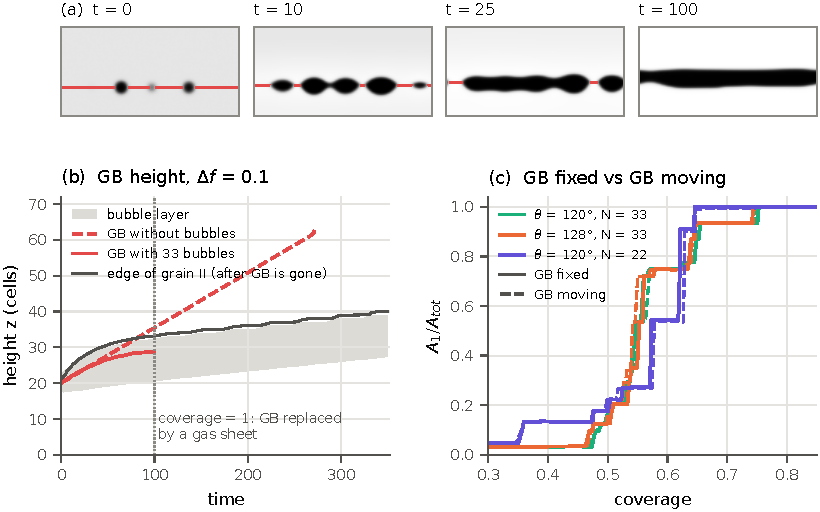
\includegraphics[width=\textwidth]{f6_coupled.pdf}
\caption{Bubbles on a moving GB ($\theta=120^\circ$, $\Delta f=0.1$).
(a)~Side cuts: black is gas, red is the GB; by $t=100$ a gas sheet has replaced
the GB. (b)~GB height over time, with and without bubbles. (c)~Percolation curve
with the GB fixed (solid) and moving (dashed) for three cases; they overlap.}
\label{fig:coupled}
\end{figure}

\begin{figure}[t]
\centering
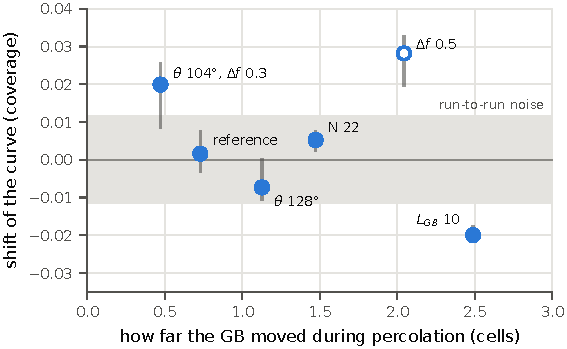
\includegraphics[width=0.6\textwidth]{f7_shift.pdf}
\caption{How much the percolation curve shifts when the GB moves, against how
far the GB moved while the bubbles were joining. Grey band: noise level (two
fixed-GB runs that differ only in GB mobility). Hollow point: $\Delta f=0.5$,
which also changes the gas behaviour.}
\label{fig:shift}
\end{figure}

\begin{takeaway}
\textbf{Take-away.} Separate bubbles do not pin a moving GB; it carries them
along. Only a continuous gas sheet stops it. The percolation curve ($A_1/\Atot$
vs coverage) is \emph{independent of GB movement}.
\end{takeaway}

% ----------------------------------------------------------------------------
\section{Step 5: towards a polycrystal}
\label{sec:poly}

Real materials have many grains, with curved GBs that meet at triple junctions.
We took two steps in that direction (Fig.~\ref{fig:poly}).

\textbf{A closed, round GB.} A spherical grain ($R_0=32$) inside another grain
shrinks because its GB is curved. Without bubbles it disappears at $t=136$
($\Delta f=0$) or 71 ($\Delta f=0.1$), close to theory. With 25 bubbles on its
GB, the bubbles again join into a closed gas shell (at $t=155$ and 99). The
shell slows the shrinking by 2.2--2.6$\times$, but the grain still disappears
(at $t=228$ and 135): unlike the flat case, a curved gas shell cannot stop a
grain.

\textbf{A 2-D polycrystal.} Earlier in the project we also wrote a
multi-grain Allen--Cahn code with 25 grains (Fig.~\ref{fig:poly}b,c). Starting
from sharp, straight boundaries, the GBs relax into smooth, curved boundaries
that meet at triple junctions. The next step is to put bubbles on this whole GB
network.

\begin{figure}[t]
\centering
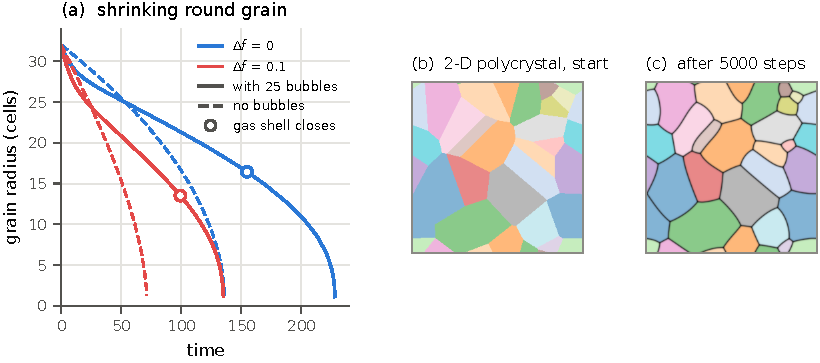
\includegraphics[width=\textwidth]{f8_poly.pdf}
\caption{(a)~Radius of a shrinking round grain with 25 bubbles on its GB (solid)
and without bubbles (dashed). (b,c)~2-D polycrystal with 25 grains at the start
and after 5000 time steps (dark lines: GBs).}
\label{fig:poly}
\end{figure}

\textbf{Ideas for the polycrystal study.}
\begin{itemize}
  \item Do bubbles prefer triple junctions, and does percolation start there?
  \item Is the percolation coverage on each GB the same as on our single flat GB?
  \item When does the gas network connect across many grains, so that gas can
        reach a free surface?
  \item How do grain growth (moving, curved GBs) and bubble percolation affect
        each other?
\end{itemize}

% ----------------------------------------------------------------------------
\section{Conclusions}

\begin{enumerate}
  \item A single bubble must be larger than about 3.5 cells to grow, and flatter
        (low-$\theta$) bubbles grow faster.
  \item For a given set of bubbles, percolation starts at the same coverage for
        all contact angles (0.39 for 33 bubbles) and ends at the same coverage for
        the angles that reach the end (0.70--0.72). The contact angle mainly
        changes the \emph{time} (up to 3.4$\times$).
  \item Fewer bubbles (25) make percolation start and end at lower coverage
        (0.32--0.34 and 0.64--0.65).
  \item Very round bubbles ($\theta\ge128^\circ$) stop connecting: islands round
        up, gaps stop closing and small islands dissolve.
  \item A flat GB moves steadily under a driving force, but the grid pins it at
        small forces.
  \item Separate bubbles do not pin a moving GB; it drags them. Only a continuous
        gas sheet stops it.
  \item The percolation curve is independent of GB movement (shift $\le0.01$ in
        coverage at normal driving forces).
\end{enumerate}

\textbf{Limitations.} We used one random bubble layout per $N$; $\theta$ is
uncertain by about $\pm6^\circ$; the high-angle runs were stopped at $t=150$; and
all results are in dimensionless units. \textbf{Next steps:} several random
layouts, a continuous gas source (ongoing irradiation), physical units for
UO$_2$ and steels, and the polycrystal study above.

\paragraph{Note on AI assistance.} An AI assistant (Claude, Anthropic) helped
draft the text of this report and the plotting script for the figures. It
worked from the author's own simulation data and notes. All simulations and
numerical results are from the author's runs.

% ----------------------------------------------------------------------------
\small
\begin{thebibliography}{9}
\setlength{\itemsep}{1pt}
\bibitem{Trinkaus2003}
H.~Trinkaus and B.~N. Singh, Helium accumulation in metals during
irradiation -- where do we stand?, \emph{J. Nucl. Mater.} \textbf{323}, 229--242 (2003).
\bibitem{Tonks2018}
M.~Tonks et al., Unit mechanisms of fission gas release: current understanding
and future needs, \emph{J. Nucl. Mater.} \textbf{504}, 300--317 (2018).
\bibitem{White2004}
R.~J. White, The development of grain-face porosity in irradiated oxide fuel,
\emph{J. Nucl. Mater.} \textbf{325}, 61--77 (2004).
\bibitem{Millett2012}
P.~C. Millett, M.~R. Tonks, S.~B. Biner et al., Phase-field simulation of
intergranular bubble growth and percolation in bicrystals,
\emph{J. Nucl. Mater.} \textbf{425}, 130--135 (2012).
\bibitem{CahnHilliard1958}
J.~W. Cahn and J.~E. Hilliard, Free energy of a nonuniform system. I.
Interfacial free energy, \emph{J. Chem. Phys.} \textbf{28}, 258--267 (1958).
\bibitem{AllenCahn1979}
S.~M. Allen and J.~W. Cahn, A microscopic theory for antiphase boundary motion
and its application to antiphase domain coarsening, \emph{Acta Metall.}
\textbf{27}, 1085--1095 (1979).
\end{thebibliography}

\end{document}
